\documentclass[slidestop,compress,mathserif, xcolor=table]{beamer}
\usepackage[T1]{fontenc}
\usepackage{lmodern}
\usepackage[utf8]{inputenc}
\usepackage[english]{babel}
\usepackage{graphicx}
\usepackage{amsmath}
\usepackage{amssymb}
\usepackage{listings}
\usepackage{enumitem}

\usetheme{Madrid}
\setbeamertemplate{headline}{}
\definecolor{scigreen}{RGB}{70,116,60}
\setbeamercolor{structure}{fg=scigreen}
\setbeamercovered{highly dynamic}
\setitemize{label=\usebeamerfont*{itemize item}
  \usebeamercolor[fg]{itemize item}
  \usebeamertemplate{itemize item}}

\title{Improving Rasterific}
\author[Chi, William]{Chi, William}
\institute[DIKU]{Department of Computer Science, University of Copenhagen}
\date{\today}

\begin{document}

\frame{\titlepage}
\begin{frame}[c]{Project}
    \begin{itemize}
    \item Rasterific is a vector drawing library; a rasteriser.
    \item Can we improve the performance of Rasterific by adding parallelism?
    \end{itemize}
\begin{figure}
\centering
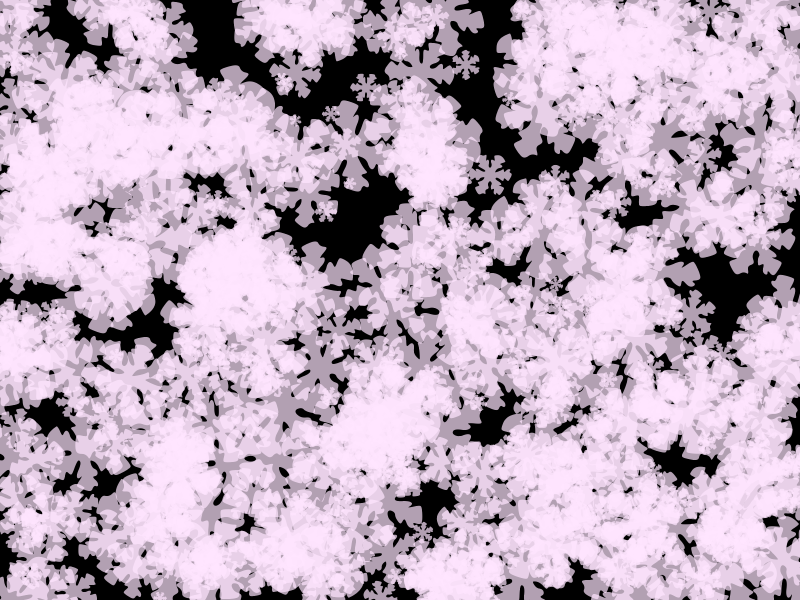
\includegraphics[width=0.3\linewidth]{../flakes}

\includegraphics[width=0.3\linewidth]{../bigsquare}
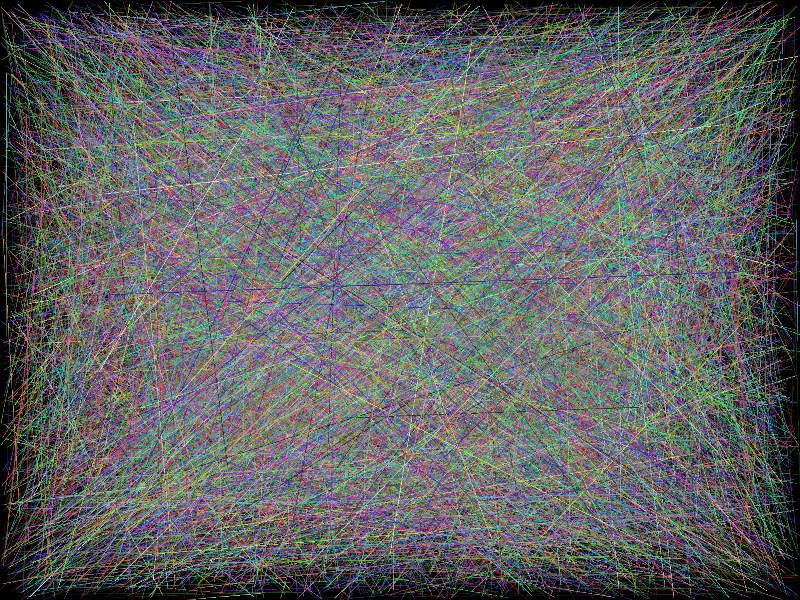
\includegraphics[width=0.3\linewidth]{../lines}
\caption{Rasterised images created by Rasterific.}
\end{figure}
\end{frame}

\begin{frame}[c]{Rasterific}
  \begin{itemize}
  \item An open source vector graphics rasteriser.
  \item Written in Haskell.
  \item No parallelism.
  \end{itemize}

\begin{figure}[h!]
  \centering
  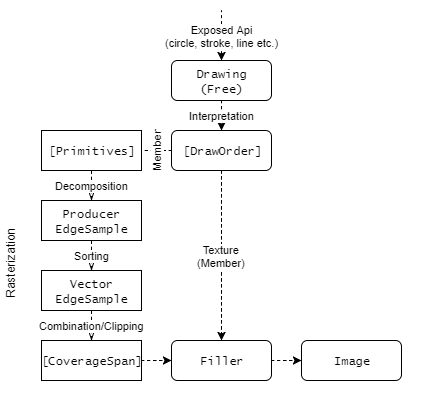
\includegraphics[width=.4\linewidth]{../rasterific-pipeline}
  \caption{Approximation of the Rasterific pipeline.}
\end{figure}

\end{frame}

\begin{frame}[c]{Experiments}
\begin{itemize}
\item 4 modular experiments in parallelising at different granularities.
\item Strict \texttt{Control.Monad.Par} for parallelism.
\end{itemize}
\begin{figure}
\centering
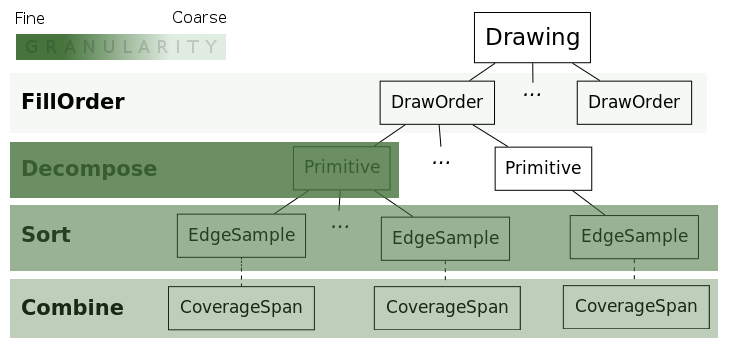
\includegraphics[width=0.9\linewidth]{../tree}
\caption{Tree structure of Rasterific with our experiments.}
\end{figure}
\end{frame}

\begin{frame}[c]{Decomposition of \texttt{Primitives}}
  \begin{itemize}
  \item Fine-grained parallelism.
  \item Simple divide-and-conquer -- straightforward implementation.
  \end{itemize}
  \begin{figure}[h!]
    \centering
    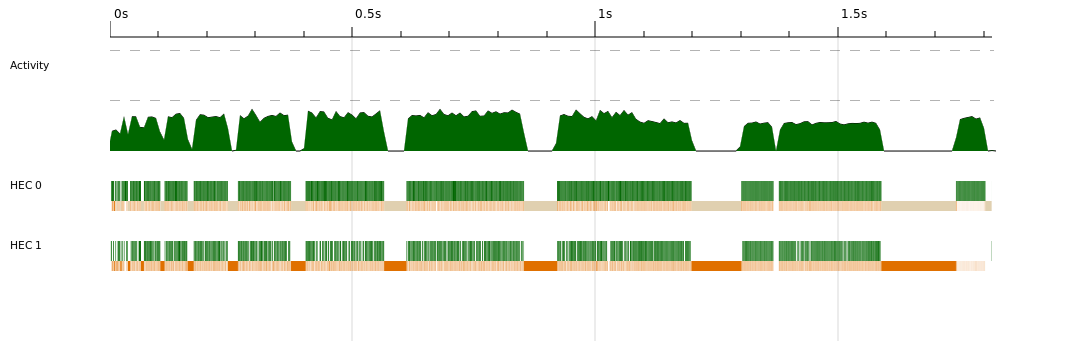
\includegraphics[width=0.7\linewidth]{../threadscope/lines/single-line-every-10}\\
    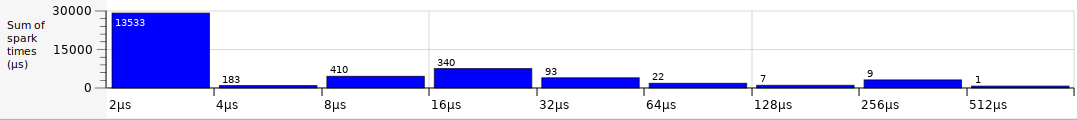
\includegraphics[width=0.7\linewidth]{../threadscope/lines/single-line-every-10-spark-times}
    \caption{ThreadScope output for decomposing a 1M px long line.}
  \label{fig:line-thread-sparks}

\end{figure}
\end{frame}
% NOTE: each experiment slide should be fairly brief during presentation -- not too many technical details, rather an explanation of parallel granularity + what we saw in threadscope
\begin{frame}[c]{Sorting \texttt{EdgeSamples}}
  \begin{itemize}
  \item Coarser-grained parallelism.
  \item Complex implementation.
  \end{itemize}
 \begin{figure}[h!]
  \centering
  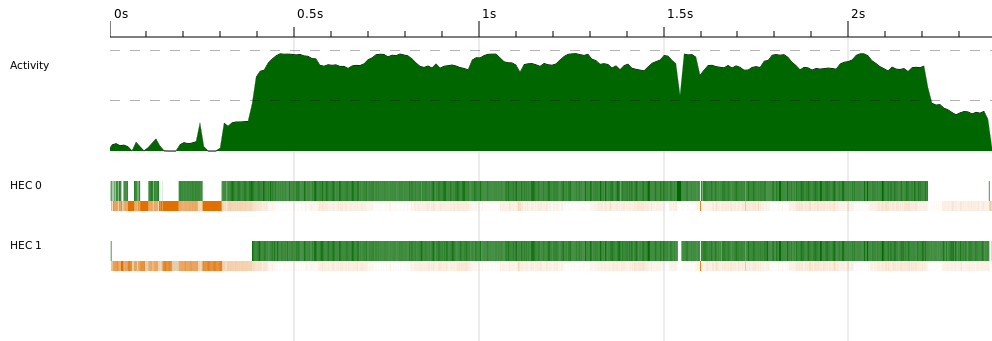
\includegraphics[width=0.7\linewidth,trim={0cm 2cm 0 0},clip]{../threadscope/sorting/sorting-final}\\
  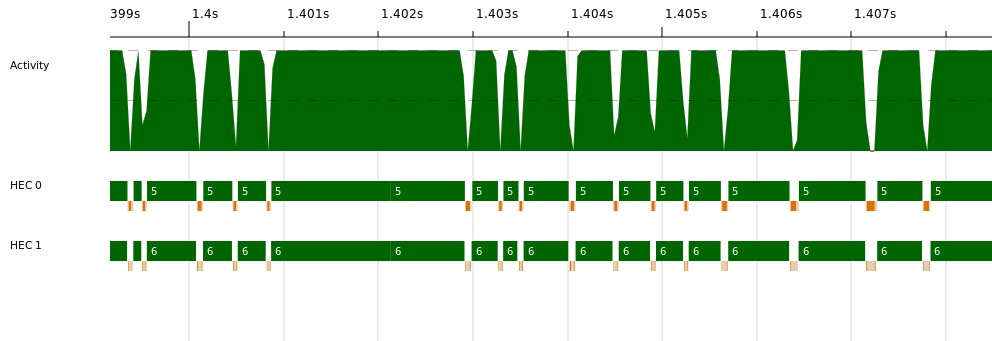
\includegraphics[width=0.3\linewidth,trim={4cm 3cm 5cm 0},clip]{../threadscope/sorting/sorting-final-zoom}
  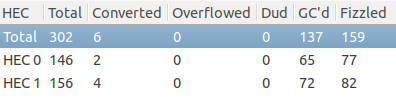
\includegraphics[width=0.4\linewidth,trim={0 0 0 1cm}]{../threadscope/sorting/sorting-final-sparks}
  \caption{ThreadScope output for sorting 1.000.000 \texttt{EdgeSample}s.}
  \label{fig:sorting-thread}
\end{figure}

\end{frame}

\begin{frame}[c]{Combining \texttt{EdgeSamples} into \texttt{CoverageSpans}}
  \begin{itemize}
  \item Parallel across rows of \texttt{EdgeSamples}.
  \item Refactoring introduces expensive conversions.
  \end{itemize}
 \begin{figure}[h!]
  \centering
  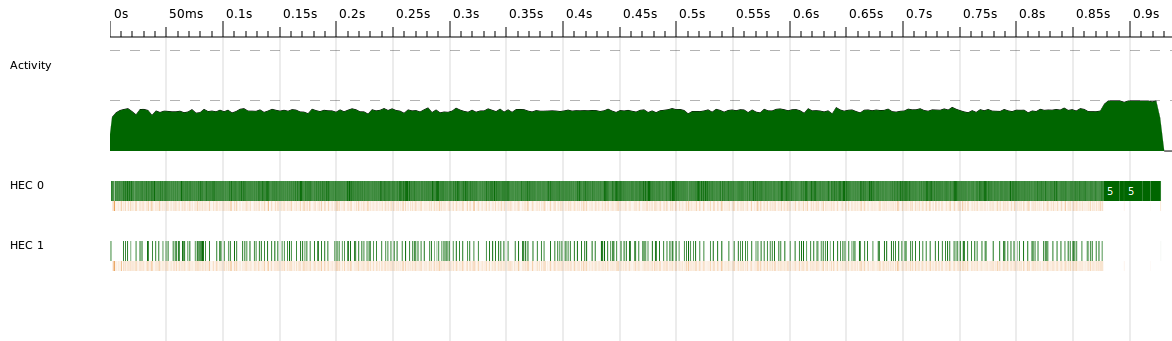
\includegraphics[width=0.7\linewidth,trim={0cm 2cm 0 0},clip]{../threadscope/combinegrouped/bigflake}\\
  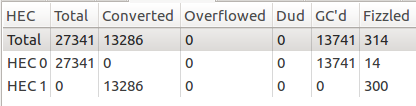
\includegraphics[width=0.55\linewidth,trim={0 0 0 0},clip]{../threadscope/combinegrouped/sparks}
  \caption{ThreadScope output for running the \texttt{snowflake} program with 500 flakes.}
\end{figure}
\end{frame}

\begin{frame}[c]{Filling \texttt{DrawOrders}}
  \begin{itemize}
  \item Coarsest level of parallelism in this project.
  \item Strict evaluation forces garbage collection.
  \end{itemize}
 \begin{figure}[h!]
  \centering
  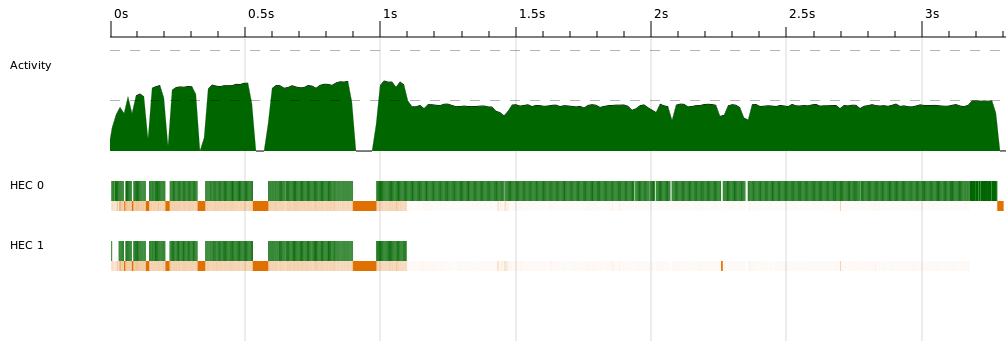
\includegraphics[width=0.7\linewidth,trim={0cm 2cm 0 0},clip]{../threadscope/fillorder/lines}\\
  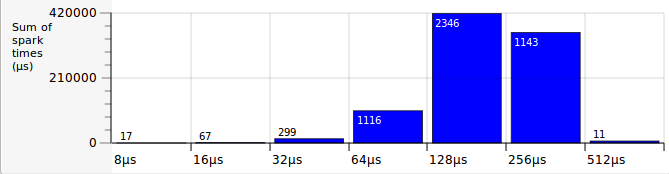
\includegraphics[width=0.3\linewidth,height=0.15\textheight,trim={0 0 0 0},clip]{../threadscope/fillorder/lines-spark-sizes}
    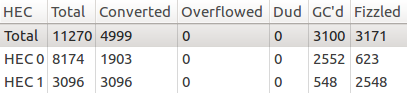
\includegraphics[width=0.4\linewidth,height=0.15\textheight,trim={0 0 0 0},clip]{../threadscope/fillorder/lines-spark}
  \caption{ThreadScope output for running the \texttt{lines} program with 5000 lines.}
\end{figure}
\end{frame}

\begin{frame}{Benchmarks and Results}

\begin{tabular}{cl}
  \begin{tabular}{l}
  \parbox{0.3\linewidth}{
  \begin{itemize}[leftmargin=0cm]
   \item \texttt{bigsquare}:\newline 1 \texttt{DrawOrder}\newline 104626 \texttt{EdgeSamples}
   \item \texttt{lines}:\newline 1000 \texttt{DrawOrders}\newline <2000 \texttt{EdgeSamples}
   \item \texttt{snowflakes}:\newline 500 \texttt{DrawOrders}\newline <2000 \texttt{EdgeSamples}
  \end{itemize}
  }
  \end{tabular} &
  \begin{tabular}{c}
  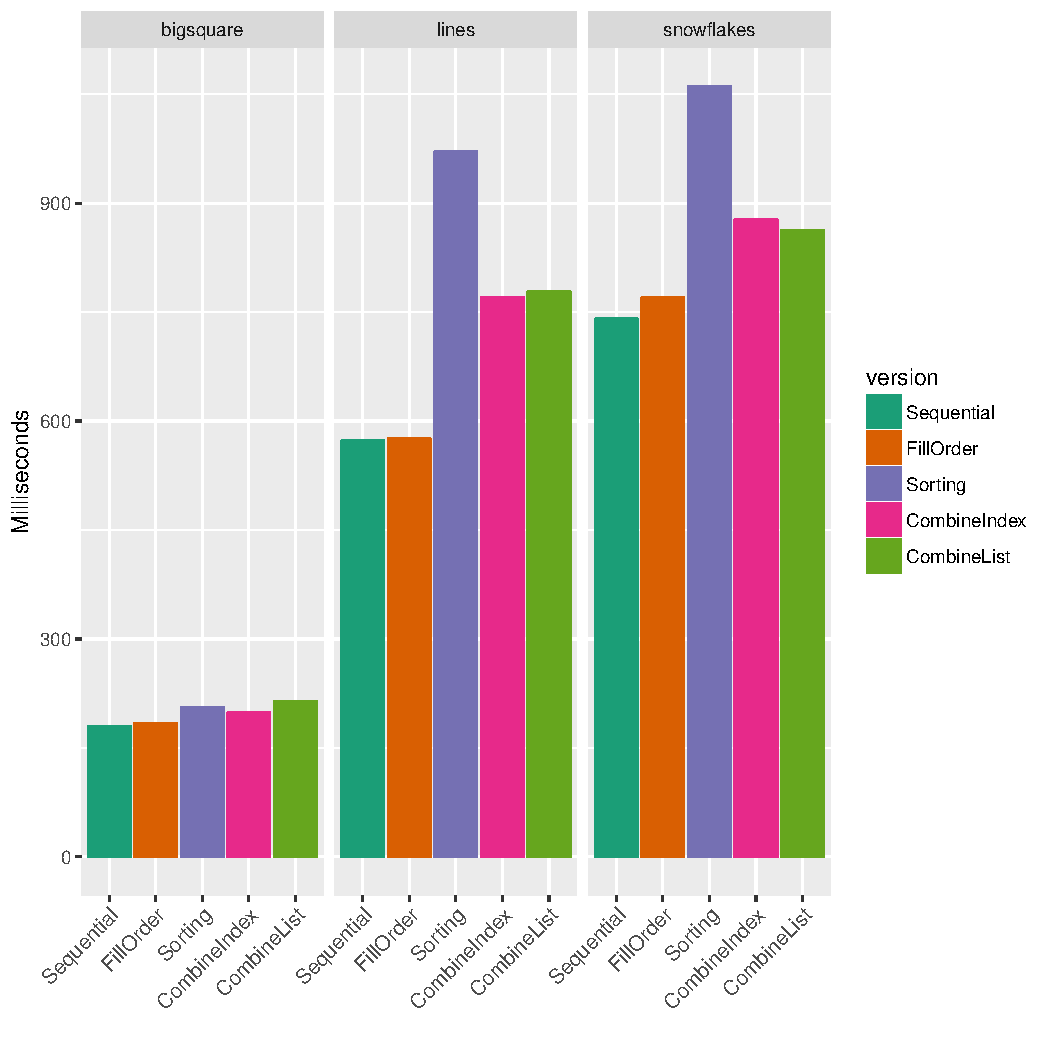
\includegraphics[width=0.6\linewidth,trim={0cm 0.5cm 0 0},clip]{../timings}
  \end{tabular}
\end{tabular}
\end{frame}

\begin{frame}[c]{Evaluation}
Original, sequential version beats all our attempts. Why?\\
\bigskip

Fine-grained parallelism:
\begin{itemize}
\item Too little work.
\item Too much overhead in data structure conversion.
\end{itemize}
\bigskip

Coarse-grained parallelism:
\begin{itemize}
\item GC overhead -- strictness causes memory strain.
\item Nested parallelism.
\end{itemize}
\end{frame}

\begin{frame}[c]{Further Work}

\begin{itemize}
\item Parallel sorting with \texttt{ST}.
\item Chunking small workloads / dynamic strategy.
\item Parallel \texttt{concatMap}.
\item Use non-strict parallelism.
\item Refactor Rasterific for strictness or flatness.
\item ...
\end{itemize}
\end{frame}

\begin{frame}[c]{Conclusion}

TL;DR: There is plenty of scope for parallelism in Rasterific, but we didn't manage to use it.

\end{frame}
\end{document}
